\section{Evaluation}

Final results of the experiment with keypoint ratio as threshold measure performs significantly better
than the keypoint count threshold measure. Hence, it can be concluded that keypoint ratio is a better
threshold measure that keypoint count.
\vspace{12pt}

There is a sudden drop of accuracies between 20\% and 50\% pitch changes. Sudden drop happens when shifting
up or down on frequency axis makes spectrogram local patterns to compressed or expanded which makes the pattern
to get unidentified as shown in the Figure \ref{fig:spectrogram_down}.


\begin{figure}[H]
    \centering
    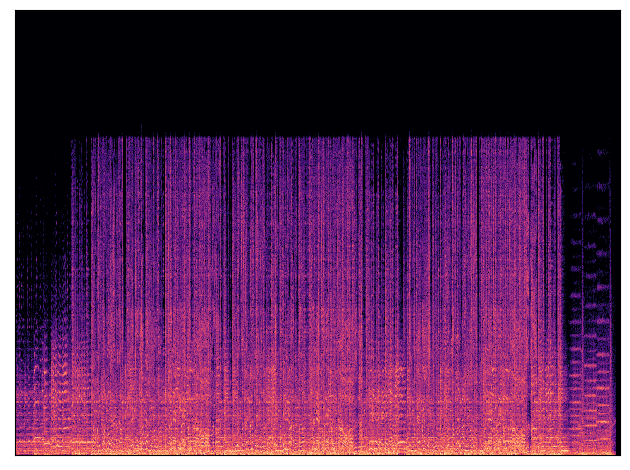
\includegraphics[scale=0.5]{spectrogram_down.png}
    \caption{Generated colour image of a spectrogram (50\% pitch decrease)}
    \label{fig:spectrogram_down}
  \end{figure}